\section{Results}
\label{sec:Results}
some introductory words

\subsection{Limits on Contribution to the HESE Flux by Transient Neutrino 
Sources}
In chapter \ref{sec:limits}, the methodology to calculate limits on the 
contribution of a transient population to the HESE flux was described. The 
pseudo experiments need to be repeated for each different signal model. The 
result for a spectrum with $\gamma=2.3$, 3000 GRBs per year and a fraction of 
5.95\% of the HESE flux to be produced by these GRBs are shown in Figures 
\ref{fig:test_statistic} and \ref{fig:test_statistic_cumulative}. The GRB rate 
density is not a known value but a parameter. To calculate the p-value for 
different rate densities and fraction of contribution to the HESE flux, the 
signal expectation $\mu_s$ can be scaled by 
\begin{equation}
 \hat{\mu_s} = \mu_s \cdot \zeta \frac{3000\mathrm{ 
GRBs/yr}}{N_\mathrm{GRBs/yr}}
\end{equation}
with $\zeta$ being the contribution to the total HESE flux. By doubling the 
number of GRBs, the neutrino flux per GRB gets reduced by half, leading to 
softer limits.

\begin{figure}[h]
 \centering
 \captionsetup{width=.9\textwidth}
%  \captionsetup{margin=0pt}
 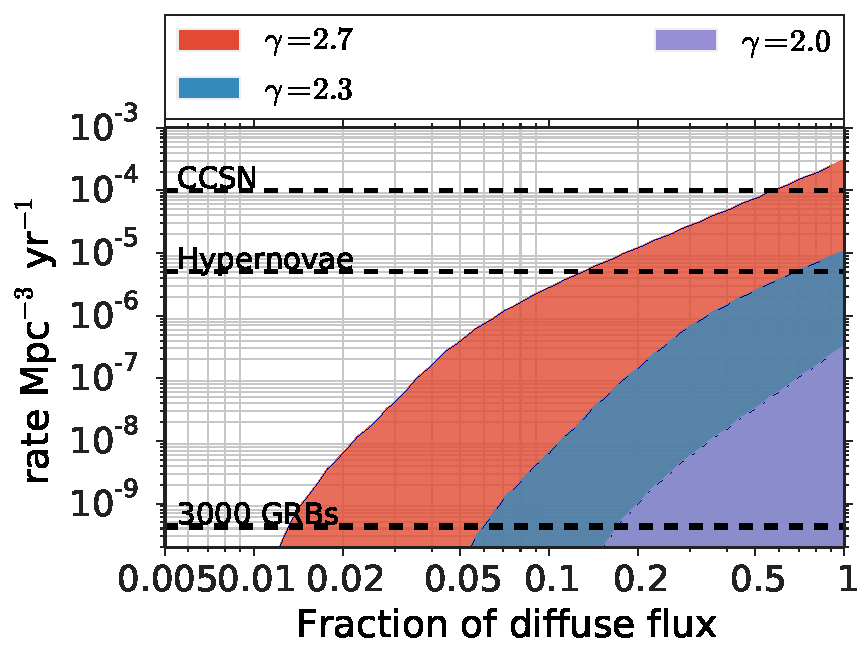
\includegraphics[width=0.75\textwidth]{fig/limits_wp_allgammas.pdf}
\caption{}
\label{fig:WP_2d_limit}
\end{figure}

Figure \ref{fig:WP_2d_limit} showcases the limits for the three different 
spectra using the WP model. The softer the spectrum the more singlets are 
expected especially at lower energies (Fig. \ref{fig:Espectra}) increase the 
multiplet expectation as well. Therefore, the hardest limits can be 
drawn using a spectrum with $\gamma=2.7$ decreasing in power the harder the 
spectrum gets. The results for a flux to be ruled out at a 90\% confidence 
level are listed in Table \ref{tab:WP_2d_limit_3000}.


\begin{table}[h]
  \centering
  \begin{tabular}{c|c|c}
$\gamma$  &  $N_\mathrm{GRB/yr}$ & $\zeta$ \\
\hline
2.7 & 3000 & 0.013 \\
2.3 & 3000 & 0.0595 \\
2.0 & 3000 & 0.18 \\
  \end{tabular}
  \caption{The values of the fraction to the HESE flux and the number of GRBs 
per year that are ruled out at a 90\% confidence level.}
  \label{tab:WP_2d_limit_3000}
\end{table}


\subsubsection{Signal origin}
As part of the analysis, the question which simulated GRBs contribute most to 
the limits, shall be answered in this section.



test statistic distribution shows the point at which p=0.9 was reached for WP 
for 3000 GRBs showing maximum contribution of 0.05\%??? (factor 0.05 on HESE 
flux -> $\mu$ <- describing the scaling in )

total number of GRBs is uncertain. therefore limits depending on the transient 
rate density and the fraction of the HESE flux are drawn. the more sources 
contribute to the known signal the less flux can be attributed to one source. 
scale $\mu (Nexp) = \mu \frac{x GRBs}{3000 GRBs}$ . limit plots

the softer the spectrum the more singlets (especially at low energies) and 
therefore more multiplets (reference spectrum plot) can be expected. 
influence of a minimal energy cutoff in section ???. best limit for gamma=2.7 
scenario. worst for gamma=2. with cutoff. some numbers (maybe in table)

looking at higher transient rates, limits extend to SN (which kind) especially 
considering that not all SN are expected to generate jets. further discussion 
in section ???.

where does signal come from? close and high. need to see plots to write more



\subsection{Different models}
So far, the Wanderman Piran model was examined to present the results of the
analysis. The influence of two different factors will be analyzed in the 
subsequent sections. 

The WP model is based on a broad luminosity function. The resulting variation 
in luminosity can lead to seldom but very bright GRBs producing the most 
detectable signal. Two different luminosity functions will be examined, the 
Howell Coward model (Section \ref{sec:results_HC}) and a more SN conform 
luminosity distribution (Section \ref{sec:results_SN}). 

The second factor is a low energy cut-off, having great influence on the final 
limits on the HESE flux contribution (Section \ref{sec:results_Emin}).

\subsubsection{Howell Coward}
\label{sec:results_HC}
The Howell Coward model (Section ???) predicts various luminosity distributions 
that have one thing in common when compared to WP: less GRBs are predicted at 
high peak luminosity values (Fig. \ref{fig:wp_hc_comp_z}). While the slope at 
low peak luminosities is with $\alpha_{WP}=???$ and $\alpha_{HC}=???$ quite 
similar,  the distributions diverge quite strongly above $L_\mathrm{Peak} \geq 
1e52 \mathrm{ erg} \mathrm{ s}^{-1}$ and the HC luminosity function drops with 
$\beta{HC}=???$ much faster than the WP function ($\beta{WP}=???$).

The impact of this deviating behavior will be examined for the flux model with 
a spectral index of $\gamma=2.3$ as the intermediate model. The result can be 
seen in Figure ???, displaying the less stringent limits of the HC model. 
Assuming 3000 contributing GRBs per year, the contribution to the HESE flux of 
GRBs following the HC luminosity can be determined at a 90\% confidence level to 
be less than ???\% (WP: ???\%).

Looking at the test statistic distributions at the 90\% exclusion value for 
each model, the low luminosity GRBs reproduce the overall distribution quite 
well (Fig. ???) in case of the HC model while one can observe a significant 
shift between the distributions - and therefore worse limits - for the WP model 
(Fig. ???). The cumulative distributions further support the result that the 
high luminosity GRBs do not contribute much to the HC-limit while each 
luminosity bin ($L_\mathrm{Peak} \in [1e52, 1e53)$ and $L_\mathrm{Peak} \in 
[1e53, 1e54]$) ????need the plots???? can still rule out the WP model at 
80\%??? confidence level.

show contribution to Luminosity, redshift??? maybe how far can I look -> more 
dependent on low lum GRBs. can not look as deep.

In conclusion it is possible to say that the limits do depend on the luminosity 
function. The limits on the HC model are mainly produced by the low 
luminosity GRBs due to the lack of high luminosity ones. This leads to 
worse limits in comparison to the WP model. However, they still exclude a wide 
region of parameter space.


\subsubsection{Supernova Luminosity Function}
\label{sec:results_SN}
redshift distribution can stay the same. or did I already write that?

for low signal: advantage trough broad Luminosity -> once in a while a very 
bright GRB -> signal

least variation: delta function. in comparison to GRB models this is the trend.

mainly gamma=2.7 reached SN sensitivity. though not number of SN considered in 
plot that actually produces a jet -> reduces the possible y-value

\subsubsection{Low Energy Cut-Off}
\label{sec:results_Emin}
emin: change normalization plot in normalization chapter with the correct one 
(Ecut HESE)


